\chapter{Hyper-Heuristics}
\label{chap:hhs}

\begin{quotation}
    \textit{``Live as if you were to die tomorrow. Learn as if you were to live forever.'' - Mahatma Gandhi}
\end{quotation}

One of the biggest challenges for any \ac{ML} researcher is that it is hard to find optimal configurations. These configurations often include the selection of appropriate models, heuristics and hyper-parameters. The optimal configuration is more often than not, problem-specific and it is difficult to find general approaches that can be applied to many situations. Traditionally, if multiple configurations are to be considered, an empirical process of trial and error is executed. Trial and error approaches are time consuming and illustrates a problem of generalisation of solutions. A modern approach to this problem is to automate this process. Automation of this process can be done by brute force where many different configurations are considered iteratively, sweeping over different configurations one after the other. Only after all configurations have been considered, can an optimal configuration be identified.

A different approach is to find optimal configurations by means of a search process. This means that a higher level optimisation process can be defined where the optimal configurations can be found as part of a search process. It is important to note that this search process is separate from the underlying problem to be solved. A measure of abstraction comes into play. In the context of training \acp{FFNN}, this is equivalent to finding the appropriate heuristic and hyper-parameters at various timesteps throughout the training process.

Automation alone is not enough. It is often the case that a single configuration is not sufficient. A modern suggestion is to include a hybridisation approach where multiple configurations are considered together. This is the nature of \acp{HH}. This is different from \textit{ensemble} \cite{ref:dietterich:2002} approaches in the sense that \acp{HH} provide a single solution, where as \textit{ensembles} make use of the combination of solutions that undergo a net weighted transformation in order to produce a final solution.

So far the reader has been presented with background information on \acp{ANN} and heuristics. This chapter aims to provide the reader with the necessary background information on \acp{HH}. It should be noted that this is a short chapter as the foundations of heuristics have already been presented in Chapter \ref{chap:heuristics}. The remainder of the chapter is structured as follows:

\begin{itemize}
    \item \textbf{Section \ref{sec:hh:meta_learning}} provides the reader with a brief definition and discussion on meta-learning.
    
    \item \textbf{Section \ref{sec:hh:what_is_a_hh}} presents the concept of a \ac{HH} and a formal definition is provided.
    
    \item \textbf{Section \ref{sec:hh:classification}} provides a detailed discussion on the classification and types of \acp{HH}.
    
    \item \textbf{Section \ref{sec:hh:application_to_nn_training}} sheds light on the applications of \acp{HH} in the context of training \acp{NN}.
    
    \item Finally, a summary of the chapter is provided in \textbf{Section \ref{sec:hh:summary}}.
\end{itemize}



\section{Meta-Learning}
\label{sec:hh:meta_learning}

Meta learning is a branch of metacognition and is concerned with learning about the learning processes. Meta-learning studies how learning systems can increase in efficiency through experience and is broadly defined as the learning process concerned with the concept of \textit{learning to learn} \cite{ref:vilalta:2002}. The goal of meta-learning is to understand if learning itself can become flexible to the problem domain or task under consideration.

\citeauthor{ref:vilalta:2002} \cite{ref:vilalta:2002} mentions that meta-learning differs from base-learning in the scope of the level of adaptation. Meta-learning is concerned with learning how to choosing the right configuration and biases dynamically. On the contrary, for \textit{base}-learning, biases and configurations are predefined and fixed a priori.


\section{What are Hyper-Heuristics?}
\label{sec:hh:what_is_a_hh}

The term \acl{HH} was first used in 1997 \cite{ref:burke:2010} and was used to describe a protocol that combines several \ac{AI} methods in the context of automated theorem proving. The term was independently used in 2000 \cite{ref:cowling:2000} to describe ``heuristics to choose heuristics''.

Formal definition of \acp{HH} is required. \citeauthor{ref:burke:2010}\cite{ref:burke:2010} defines \acp{HH} as search methods or learning mechanism for selecting or generating heuristics to solve computational search problems. Burke goes on to say that \ac{HH} is a high-level approach that, given a particular problem instance and a number of low-level heuristics, can select and apply an appropriate low-level heuristic at each decision point \cite{ref:burke2003}. 

\citeauthor{ref:grobler:2015} \cite{ref:grobler:2015} states that \acp{HH} promote the design of more generally applicable search methodologies and tend to performing relatively well on a large set of different problems. This is in contrast to specialised algorithms which typically focus on outperforming the state-of-the-art for a single application.

Importantly, \ac{HH} are concerned with finding the best heuristic in heuristic-space, while the underlying low-level heuristics find solutions in the feasible search space. This level of abstraction is illustrated in Figure \ref{fig:heuristics:hh:hh_algorithm} below.

\begin{figure}[htbp]
    \begin{centering}
        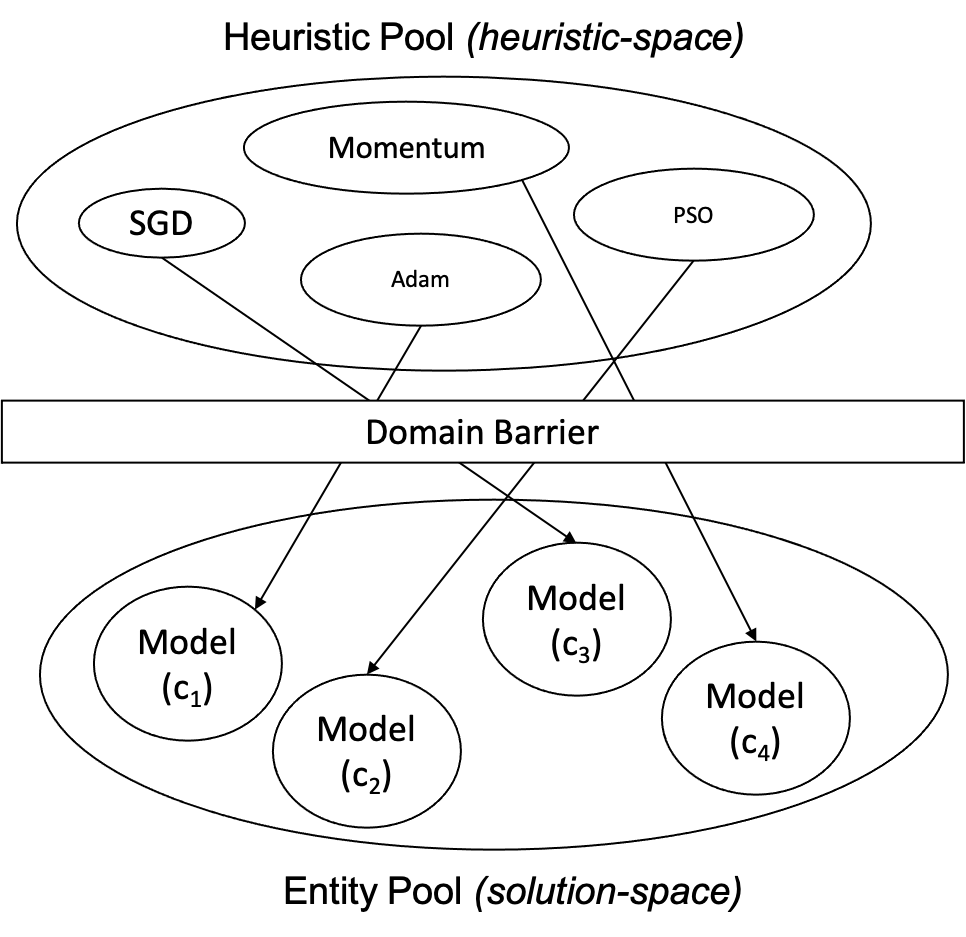
\includegraphics[width=0.8\textwidth]{images/hh_high_level.png}
        \caption{An illustration of abstraction introduced by \acp{HH}.}
        \label{fig:heuristics:hh:hh_algorithm}
    \end{centering}
\end{figure}

One can clearly see from Figure \ref{fig:heuristics:hh:hh_algorithm} the abstraction of the heuristic search process. The two large elliptical figures highlight the entity and heuristic pools, each of these are concerned with their own optimisation process. Note, that at the higher level abstraction, \acp{HH} do not make use of domain specific information such as an entity's position or gradient in the search space.

\citeauthor{ref:grobler:2015}\cite{ref:grobler:2015} mentions that two fundamental ideas behind the notion of \ac{HH} can be identified. Firstly, the recognition that the process of selecting or designing efficient hybrid and/or cooperative heuristics can be regarded as a computational search problem in itself. Secondly, there is significant potential to improve search methodologies by the incorporation of learning mechanisms that can adaptively guide the search. These two fundamental ideas have inspired different types of hyper-heuristics \cite{ref:burke:2010}.


\section{Classification of Hyper-Heuristics}
\label{sec:hh:classification}

\citeauthor{ref:burke:2010}\cite{ref:burke:2010} proposed a modern classification scheme used to classify \acp{HH}. According to the proposed classification scheme, \acp{HH} are classified in two dimensions. These include the nature of the heuristic search space and the source of feedback during learning. Figure \ref{fig:heuristics:hh:classification} was taken from \cite{ref:burke:2010} and summarises the classification scheme for \ac{HH}.

\begin{figure}[htbp]
    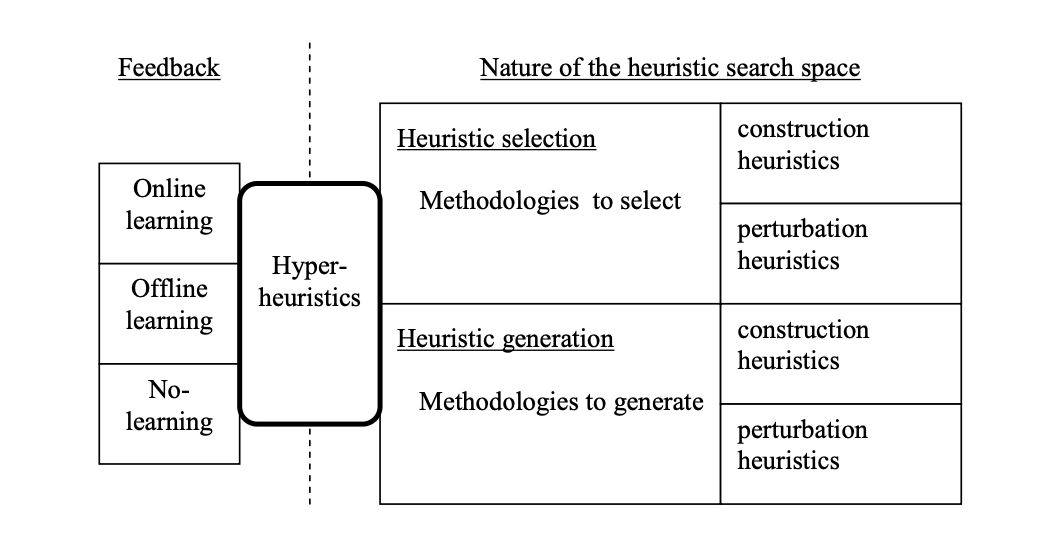
\includegraphics[width=\textwidth]{images/hh_classification.png}
    \caption{A classification of \ac{HH} approaches, according to two dimensions: (i) the nature of the heuristic search space, and (ii) the source of feedback during learning.}
    \label{fig:heuristics:hh:classification}
\end{figure}

Each of these groups are briefly discussed next.

\subsection{Selection vs. Generation}

According to the classification proposed by \cite{ref:burke:2010}, the first dimension of classification involves the nature of the search space. Distinction is made between heuristic selection and heuristic generation. For heuristic selection \acp{HH}, methodologies are implemented for choosing or selecting existing low-level heuristics. On the contrary, for heuristic generation \acp{HH}, methodologies  are implemented for generating new heuristics from components of existing heuristics.

Selection mechanisms can include probabilistic methods as is introduced in this dissertation or even some high level \ac{MH}. For generation mechanisms, \ac{EA} are often used \cite{ref:burke:2010}.

\subsection{Construction vs. Perturbation}

The second dimension of classification distinguishes between construction heuristics and perturbation heuristics. Consider first construction heuristics. According to \citeauthor{ref:burke:2010}\cite{ref:burke:2010}, these approaches build a solution incrementally. Starting with an empty solution, the goal is to intelligently select and use construction heuristics to gradually build a complete solution. As such, the \ac{HH} framework is provided with a set of pre-existing construction heuristics. These heuristics are generally problem specific and the challenge is to select the heuristic that is somehow the most suitable for the current problem state. This process is repeated until some final state such as a complete solution, is obtained.

Perturbation heuristics refer to approaches that start with a complete solution, generated either randomly or using simple construction heuristics.  Perturbation heuristics try to iteratively improve the current solution. As such, the hyper-heuristic framework is provided with a set of neighbourhood structures and/or simple local searchers. The goal here it to iteratively select and apply them to the current complete solution. This process continues until a stopping condition has been met. Notice that these approaches do not have a natural termination condition.
This is one of the biggest differences between construction and perturbation heuristics. 

\begin{itemize}
    \item (i) low-level heuristic selection, and
    \item (ii) move acceptance strategy. 
\end{itemize}

Heuristic selection can be done in a \textit{non-adaptive} or simple way. This is done either randomly or along a cycle and is based on a prefixed heuristic ordering \cite{ref:cowling:2000}. No learning is involved in these approaches. As an alternative, heuristic selection may incorporate an \textit{adaptive}, \textit{online learning}) mechanism based on the probabilistic weighting of the low-level heuristics \cite{ref:burke:2003} or some type of performance statistics \cite{ref:cowling:2000}. It will later be shown that the proposed \ac{BHH} implements this adaptive selection, perturbation strategy. 

The acceptance strategy is an important component of any local search heuristic. \cite{ref:burke:2003} mentions that many acceptance strategies have been explored within \acp{HH}. Move acceptance strategies can be divided into two categories. These include \textit{deterministic} and \textit{non-deterministic}. In general, a move is accepted or rejected, based on the quality of the move and the current solution during a single point search. At any point in the search, deterministic move acceptance methods generate the same result for the same candidate solution(s) used for the acceptance test. However, a different outcome is possible if a non-deterministic approach is used. If the move acceptance test involves other parameters, such as the current time, then these strategies are referred to as non-deterministic strategies \cite{ref:burke:2003}. 

\subsection{Online Learning vs. Offline Learning vs. No Learning}

A \ac{HH} is considered to be a learning algorithm when it uses some feedback from the search process. Therefore, non-learning hyper-heuristics are those that do not use any feedback. 

With online learning \acp{HH}, learning continues to takes place while the algorithm is solving an instance of the underlying optimisation problem. Task-dependent local properties can be used by the high-level strategy to determine the appropriate low-level heuristic to apply. Examples of online learning approaches within hyper-heuristics include the use of reinforcement learning for heuristic selection and, generally, the use of \acp{MH} as high-level search strategies across a search space of heuristics.

W.r.t offline learning \acp{HH} algorithms, the idea is to gather knowledge in the form of rules or programs, from a set of training instances. The hope is that it would generalise to the process of solving unseen instances. Examples of offline learning approaches within hyper-heuristics include \textit{learning classifier systems}, \textit{case-based reasoning} and \textit{genetic programming}.


\section{Application to Neural Network Training}
\label{sec:hh:application_to_nn_training}

Training of \ac{FFNN} is notorious for being sensitive to configurations made beforehand. \acp{HH} provide a dynamic framework to train \ac{FFNN}. However, at the time of writing, only two examples of published work where found where \ac{HH} are used for training \ac{FFNN}. These include the works of Nel \cite{ref:nel:2021} and Ul et al. \cite{ref:ul:2018}


\section{Summary}
\label{sec:hh:summary}

This chapter provided the reader with the necessary background information on \acp{HH}. A discussion on meta-learning is provided. The definition of a \ac{HH} is given and modern classifications of \ac{HH} types was discussed in detail. It was shown that \ac{HH} can be used to train \acp{FFNN}. 

This chapter then concludes the background information of heuristics in general. The next chapter aims to provide the reader with the necessary background information on statistics and probability theory. These concepts are required in order to formulate the proposed \ac{BHH}.